\section{Simulation}\label{app:simulation}

The following series of screenshots are taken from the simulation environment, where the task is to navigate to and grasp a target fish-like object with parallel jaw gripper.

\begin{figure}
\centering
\begin{subfigure}[t]{0.33\textwidth}
\centering
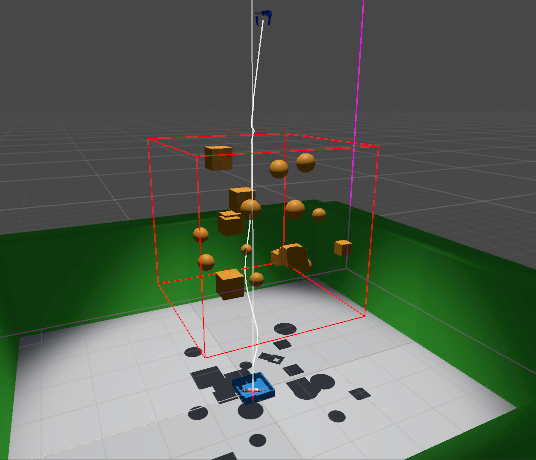
\includegraphics[width=\linewidth]{figures/simulation/editor}
\end{subfigure}%
    \hfill
\begin{subfigure}[t]{0.33\textwidth}
\centering
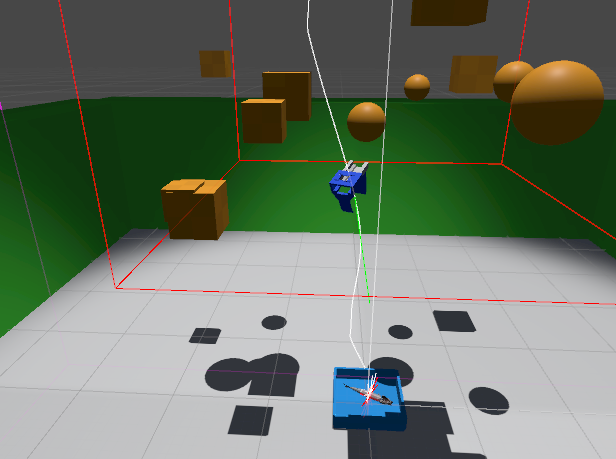
\includegraphics[width=\linewidth]{figures/simulation/editor-mid}
\end{subfigure}%
    \hfill
\begin{subfigure}[t]{0.33\textwidth}
\centering
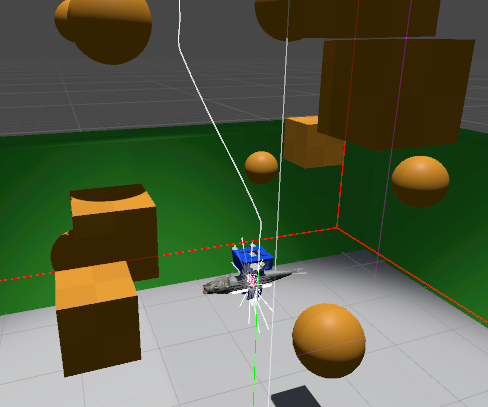
\includegraphics[width=\linewidth]{figures/simulation/editor-back}
\end{subfigure}
\caption{This figure demonstrates navigation in the environment, the thin colored lines can be displayed for development and debug purposes}
\end{figure}

\begin{figure}
\centering
\begin{subfigure}[t]{0.5\textwidth}
\centering
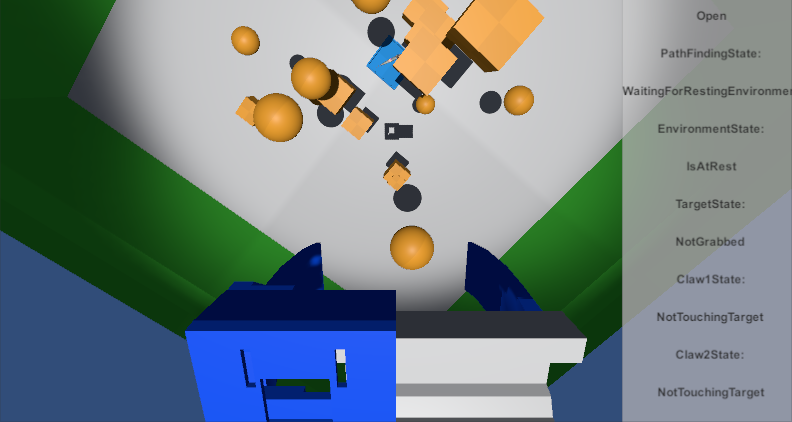
\includegraphics[width=\linewidth]{figures/simulation/game-start}
\end{subfigure}%
    \hfill
\begin{subfigure}[t]{0.5\textwidth}
\centering
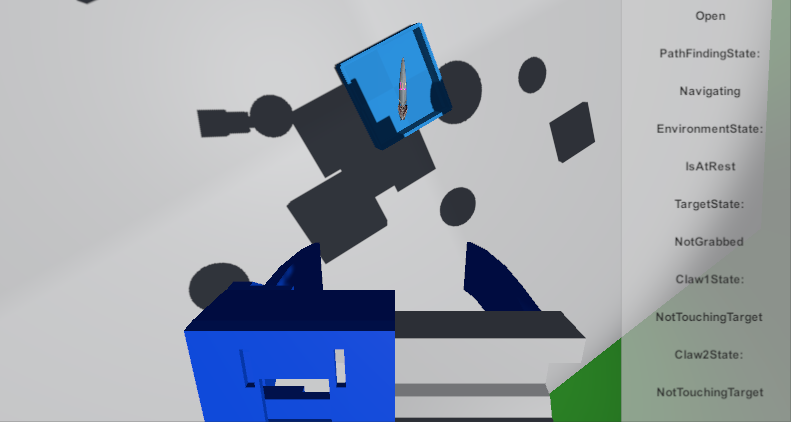
\includegraphics[width=\linewidth]{figures/simulation/game-mid}
\end{subfigure}
\\
\begin{subfigure}[t]{0.5\textwidth}
\centering
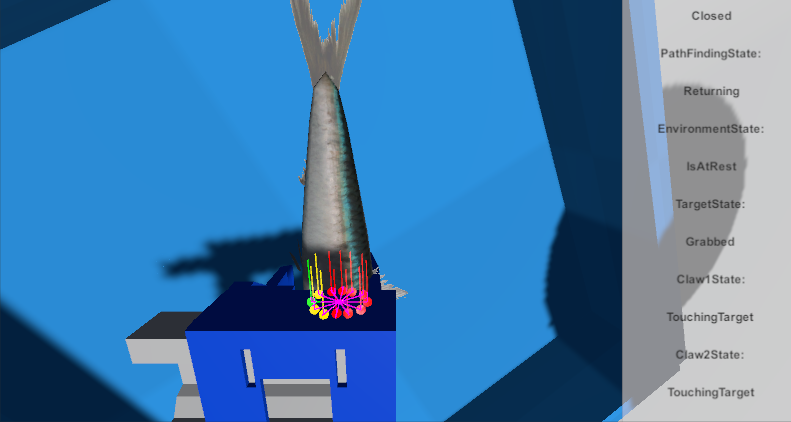
\includegraphics[width=\linewidth]{figures/simulation/grabbed}
\end{subfigure}%
\begin{subfigure}[t]{0.5\textwidth}
\centering
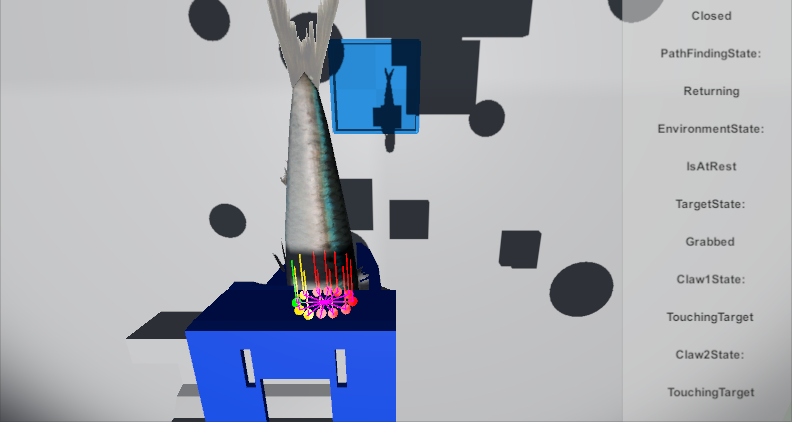
\includegraphics[width=\linewidth]{figures/simulation/returning}
\end{subfigure}
\caption{This figure are screenshots from the simulation running from the gripper perspective, this is not related to collection of training data but is useful for debugging are it thus it display current states of the simulation, as described in section~\ref{sec:states}.}
\end{figure}

\begin{figure}
\centering
\begin{subfigure}[t]{0.33\textwidth}
\centering
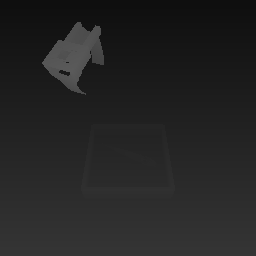
\includegraphics[width=\linewidth]{figures/simulation/depth-in}
\end{subfigure}%
    \hfill
\begin{subfigure}[t]{0.33\textwidth}
\centering

\includegraphics[width=\linewidth]{figures/simulation/depth-grabbing}
\end{subfigure}%
    \hfill
\begin{subfigure}[t]{0.33\textwidth}
\centering

\includegraphics[width=\linewidth]{figures/simulation/grabbed-depth}
\end{subfigure}
\caption{This figure are just few samples from the depth image data collected during the simulation.}
\end{figure}